\documentclass{article}
\usepackage{../CV}

\title{Josef Utbult - CV}

\begin{document}
%
\maketitle
%
\specialtext{
	Jag är en civilingenjörsstudent inom datateknik på Luleå Tekniska Universitet som kommer ifrån Öckerö utanför Göteborg. 
	Mina största intressen är musik, elektronik och programmering på både låg och något högre nivå.
}
%
\section{Kontakt}
%
% Force image to be placed to the right of the contact info, and not wrap any of the following
% lines, as the first lines outside of tables appear on the next page
\begin{wrapfigure}[0]{r}{0.3\textwidth}
	% Ugly fix to transform the image upwards
	\vspace*{-3cm}
    \centering
    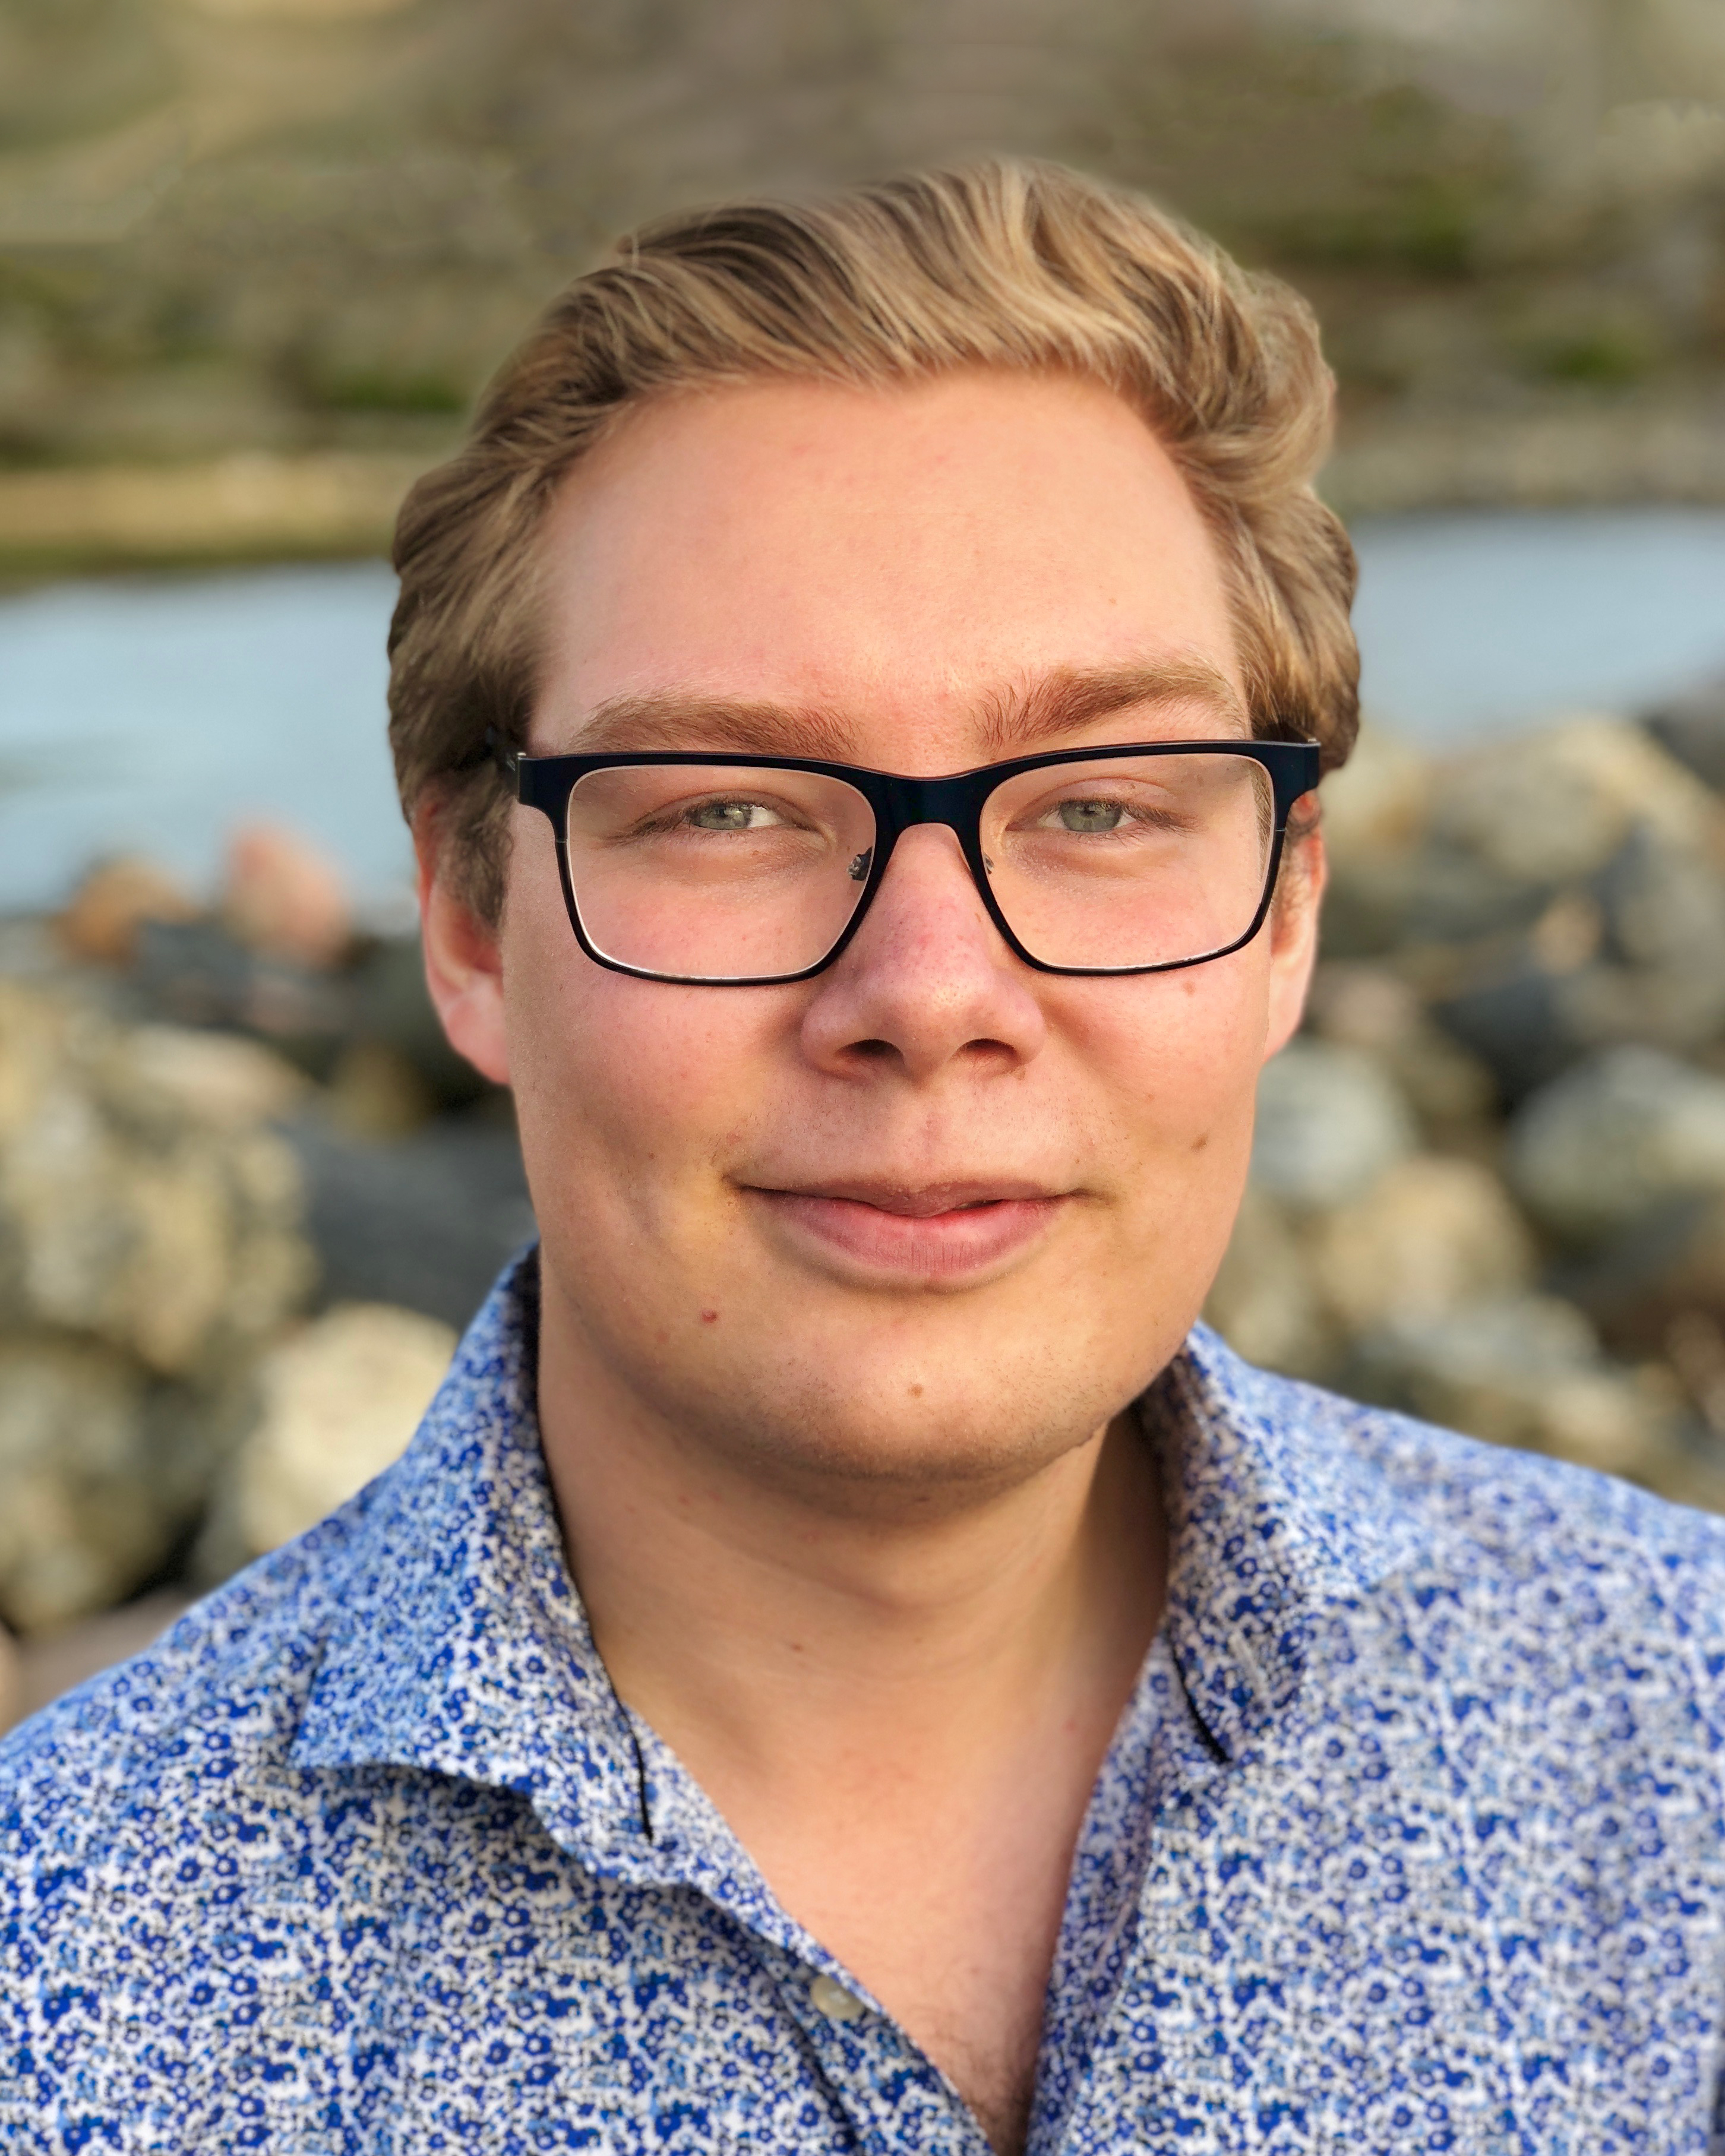
\includegraphics[width=0.26\textwidth]{profilbild.jpg}
\end{wrapfigure}%
%
\begin{tabular}{P{0.17\textwidth} P{0.30\textwidth}}
%
	Namn 			& Josef Utbult 											\\
    Födelsedadum 	& 970326 												\\
    Adress 			& Professorsvägen 21, 977 51 Luleå 						\\
    Telefonnummer 	& +46763065186   										\\
    E-post 			& \url{josef@utbult.design}								\\
	GitHub			& \url{www.github.com/JosefUtbult}						\\
    LinkedIn        & \url{www.www.linkedin.com/in/josef-utbult-969303132} 	\\
%
\end{tabular}
%
\section{Arbetserfarenhet}

\employer{Flexbridge AB}
\employmentperiod{2020 - 2022}
\subsection{Embeddedutvecklare}
Under mina studier har jag jobbat deltid sedan 2020 som embeddedutvecklare för \textit{Flexbridge AB}
\footnote{Flexbridge AB: \url{www.flexbridge.se/}}. 
Där har jag varit del i att skapa den produkt som de kallat \textit{Iceblock}, vilket är ett distribuerat styrsystem 
gjort för industriella applikationer.

Min roll har varit att skapa specialbyggda linuxdistributioner för deras specifika behov med hjälp av byggsystemen 
\textit{Buildroot} och \textit{OpenWRT}. 
Detta inkluderade egenbyggda drivrutiner skrivna i \textit{C} för att integrera deras externa komponenter med linuxkerneln samt att 
implementera deras \textit{Iceblocks} i \textit{NxT Technology IDE}, vilket är en utvecklingsmiljö för industriella system.

Jag har även implementerat \textit{Flexbridges} system för att generera och distribuera uppdateringar för deras olika produkter.

\reference{Referens: Dmitrii Drozdov (\url{dd@flexbridge.se})}

\employer{Luleå Tekniska Universitet}
\employmentperiod{Sommaren 2022 - Hösten 2022}
\subsection{Research Trainee}
Sommaren 2022 arbetade jag på \textit{Luleå Tekniska Universitet} som \textit{Research Trainee}. Jag arbetade i \textit{LTUs AIC3 labb}, 
vilket är en experimentell demonstratör av \textit{Industrial Internet}-fördelarna för \textit{Industry 4.0}\footnote{AIC3 labbet på 
Luleå Tekniska Universitet: 
\url{www.ltu.se/research/subjects/Kommunikations-och-berakningssystem/AIC3lab-Advanced-Industrial-Computing-Communication-and-Control}}.

Min uppgift under sommaren var att implementera ett styrsystem vars komponenter kommunicerade över en 5G anslutning. 
Detta gjorde jag igenom att bygga en linuxbaserad styrenhet kopplad till ett 5G modem. Denna styrenhet kopplades till ett separat meshnätverk
av styrenheter och fungerade som en accesspunkt till dessa.
Trafiken från detta meshnätverk och det nätverk resterande enheter var kopplade till routades sedan mellan dessa igenom en VPN tunnel, för att 
tillåta alla enheter att kommunicera med varandra.

Detta job gav mig bättre insikt i hur nätverk i linux fungerar, samt shell scripting och python.

\reference{Referens: Valeriy Vyatkin (+46722432592)}

\employer{Luleå Tekniska Universitet}
\employmentperiod{Hösten 2018}
\subsection{Handledare}
Hösten 2018 jobbade jag deltid under mina studier med att vara handledare för kursen \textit{Introduktion till programmering} under
\textit{Institutionen för system- och rymdteknik} vid \textit{Luleå Tekniska Universitet}. Min uppgift var att handleda studenter under de labbpass
som ingick i kursen. Detta gjorde jag främst då jag tycker om att undervisa och det har hjälpt mig med min förståelse för pedagogik och utlärande 
inom grundläggande programmering.

% TODO: Kolla med Fredrik
\reference{Referens: Fredrik Bengtsson (+46920492431)}

\employer{Musikskolan.se}
\employmentperiod{Sommaren 2018}
\subsection{Webbutvecklare}
Sommaren 2018 arbetade jag för \textit{Musikskolan.se} som producerar läromedel för musik samt säljer notböcker, musikinstrument och mjukvara.
Min uppgift var att implementera en vidospelare för deras hemsida där användare har tillgång till att se videolektioner 
tillhörande de läromedel \textit{Musikskolan.se} distribuerar.

% TODO: Hitta Pias nummer
\reference{Referens: Pia Åhlund (-)}

\newpage

\section{Utbildning}
\begin{tabular}{p{0.17\textwidth} p{0.35\textwidth} p{0.4\textwidth}}
    2017 - 		&	Civilingengör, Datateknik	& Luleå Tekniska Universitet 	\\
    2013 - 2016 &	Naturvetenskapsprogrammet	& Öckerö Seglande Gymnasieskola \\
\end{tabular}
%
\section{Övriga meriter}
\begin{tabular}{p{0.17\textwidth} p{0.35\textwidth} p{0.4\textwidth}}
    2021 - 2022 & Vice Lagchef				& Trubadurlaget STUK 												\\
    2019 - 2020 & Styrelseledamot	 		& LUDD - Luleå Tekniska Universitets Dataförening					\\ 
    2018 - 		& Kassör/Webmaster			& Frispel - Musikförening/replokal på Luleå Tekniska Universitet	\\ 
    2017 		& B-körkort 				&																	\\ 
    2013 		& Basic Safety utbildning  	& Öckerö Seglande Gymnasieskola
	%2011 - 2017 &   Scoutledare & Nimbus Öckerö Missionsförsamling \\ \\
\end{tabular}
%
\section{Erfarenheter}
Jag har erfarenhet i \textit{Python}, \textit{C++} och \textit{C}, \textit{C\#}, \textit{Javascript}, \textit{Rust} och assembler. 
Jag har utvecklat PCB:er både för professionellt och eget bruk, och har grundläggande förståelse för elektronik.
Under mitt tidigare arbete har jag arbetat med \textit{Linuxkerneln} och skrivit drivrutiner i \textit{C}.
Mitt jobb var även att bygga systemet för att skapa och distribuera uppdateringar till deras produkter.
Jag har även utvecklat i \textit{C++} för \textit{ATMega} och \textit{STM32} mikrokontrollers. Jag har grundläggande kunskap inom webbutveckling,
och har utvecklat system i \textit{Flask}, \textit{Django}, \textit{NodeJS} och \textit{MySQL}. En webbplats jag har utvecklat och 
underhåller är musikföreningen Frispels bokningssystem\footnote{Musikföreningen Frispels bokningssystem: \url{www.frispel.rocks/}}.
Jag gillar att bygga saker i \textit{Fusion360}, 3D-printing och hobbyelektronik.
\newpage
%
\section{Om mig}
Jag är positiv och har lätt för att engagera mig och ta ansvar. 
Om det behövs kan jag ta en ledande roll, men är lika bekväm med att följa direktiv. 
Jag har arbetat på distans och ansvarat för mina arbetsuppgifter under en längre tid, då jag tenderar att vara mycket självgående.
Jag blir lätt intresserad av det mesta och tar mig an allt jag kommer över.
På fritiden spelar jag gärna elbas, synthbas, trumpet och sjunger.

Jag tar mig an många projekt som brukar kretsa kring obskyra instrument och effektpedaler, men även vissa icke musikrelaterade saker.
På det senaste har jag byggt en tresträngad resebas av en shortscalegitarr, en MIDI-Guitarherokontroll för att spela Livin' on a Prayer
live och en del webbsidor. För tillfället försöker jag få ihop en pongdator av en Z80 processor samt en EEPROM.
\end{document}
%
\end{document}
